\documentclass[ignorenonframetext,xcolor=x11names]{beamer}

\input{../common.preamble.beamer.tex}

\title{Business 4720 - Class 20}

\subtitle{Analytics at Industrial Scale -- Big Data Analytics}

\begin{document}

\begin{frame}{}
  \titlepage
  \footnotesize
  \input{../license.tex}
\end{frame}

\section{Introduction}

\begin{frame}{This Class}

\begin{block}{What You Will Learn:}
\begin{itemize}
  \item Distributed data storage
  \begin{itemize}
     \item Hadoop HDFS
  \end{itemize}
  \item Distributed computation
  \begin{itemize}
     \item Hadoop Map-Reduce
     \item Spark
     \begin{itemize}
        \item Dataframe operations
        \item Spark SQL
        \item Spark MLLib
     \end{itemize}
   \end{itemize}
\end{itemize}
\end{block}
\end{frame}

\begin{frame}{Further Reading}
\begin{block}{}
Hrishikesh V. Karambelkar (2018) \emph{Apache Hadoop 3 Quick Start Guide}. Packt Publishing. Birmingham, UK.
\end{block}

\begin{block}{}
Tom White (2012) \emph{Hadoop -- The Definitive Guide}. 3rd edition. O'Reilly Media. Sebastopol, California, US.
\end{block}

\begin{block}{}
Bill Chambers and Matei Zaharia (2018) \emph{Spark -- The Definitive Guide}. O'Reilly Media. Sebastopol, California, US.
\end{block}

\begin{block}{}
Jules Damji et al. (2020) \emph{Learning Spark -- Lightning-Fast Data Analytics}. 2nd edition. O'Reilly Media. Sebastopol, California, US.
\end{block}
\end{frame}

\begin{frame}{Big Data}
Characterized by any one or more of:
\begin{itemize}
    \item Large volume
    \item Large ''velocity'' (volume per time)
    \item Large variety (of data types and sources)
\end{itemize}
\end{frame}

\begin{frame}{Big Data Example -- CERN}
''Conseil Europeenne pour la Recherche Nucleaire'' \\

\begin{center}
\includegraphics[width=.8\textwidth]{cern1.jpg} \\

\footnotesize{Source: \url{https://www.home.cern/science/computing/data-centre}}
\end{center}

\end{frame}


\begin{frame}{Big Data Example -- CERN}
''Conseil Europeenne pour la Recherche Nucleaire'' \\

\footnotesize\url{https://www.home.cern/science/computing/data-centre}\footnote{Accessed Feb 23, 2024}\small
\begin{center}
\renewcommand{\arraystretch}{1.5}
\begin{tabular}{l r l} \hline
Servers & $\approx 12000$ \\
CPU Cores & $\approx 330000$ \\
Disks & $\approx 220000$ \\
Total Disk Space & $\approx 950000$ & TB \\ 
DB Transactions per second & $\approx 20000$ \\ 
File Transfer Throughput & $\approx 500000$ & Gb/s\\  \hline
\end{tabular}
\end{center}
\end{frame}

\begin{frame}{Distributed Data and Distributed Computation}
\begin{block}{Hadoop}
\begin{itemize}
   \item Initial release 2006
   \item Maintained by the Apache Foundation
   \item Inspired by Google File System (GFS) (2003) and Google MapReduce (2004) for large data management
   \item Early use cases by Yahoo (2009) and Facebook (2012) drove adoption
   \item Distributes data storage and computation across a cluster of computers
   \item \emph{Data locality} means moving computation to data, not data to computation
\end{itemize}
\end{block}
\end{frame}

\begin{frame}{Hadoop Benefits}
\begin{itemize}
  \item \textbf{Reliability}: Hardware and software failure tolerance through replication and automatic recovery
  \item \textbf{Scalability}: Dynamically adding and removing storage nodes and cluster re-balancing (more than 10,000 nodes in Hadoop 3)
  \item \textbf{Cost effective}: Open source, runs on commodity hardware, can use heterogenous nodes
  \item \textbf{Cloud support}: Vendors offering turn-key Hadoop systems
\end{itemize}
\end{frame}

\begin{frame}{Main Hadoop Components}
\begin{itemize}
    \item \textbf{HDFS}: Hadoop Distributed File System
    \item \textbf{MapReduce}: Software framework for processing large data volumes
    \item \textbf{YARN}: Yet Another Resource Negotiator (cluster and compute job manager)
\end{itemize}

\centering
\vspace{2\baselineskip}
\includegraphics[width=.8\textwidth]{Apache_Hadoop.png}
\scriptsize \url{https://commons.wikimedia.org/wiki/File:Apache_Hadoop.png}
\end{frame}

\begin{frame}{HDFS Principles}
\begin{itemize}
   \item \textbf{Streaming data access}: Data is written and read linearly, processed one item at a time
   \item \textbf{Large datasets}: Multiple gigabytes or terabytes, hundreds of computers per clusters, millions of files per node
   \item \textbf{Write once}: Files once written are only read or appended to
   \item \textbf{Moving computation is cheaper than moving data}: Move compute applications to the server that stores the data
\end{itemize}
\end{frame}

\begin{frame}{HDFS Architecture}
\centering

\includegraphics[width=\textwidth]{hdfsarchitecture.png}
\scriptsize Source: Apache Foundation (\url{https://hadoop.apache.org/docs/})
\end{frame}

\begin{frame}{HDFS Architecture}
\begin{block}{NameNode}
\begin{itemize}
    \item One NameNode per cluster (plus sercondary/backup)
    \item Manages file namespace (sub-directories, file names, etc.)
    \item Regulates access to files
    \item Provides file operations such as opening, closing, renaming, etc.
\end{itemize}
\end{block}

\begin{block}{DataNode}
\begin{itemize}
   \item Files are split into blocks stored on DataNodes
   \item DataNodes handle read and write requests of clients
   \item DataNodes perform block operations for file operations by NameNode
\end{itemize}
\end{block}
\end{frame}

%\begin{frame}{HDFS Replication}
%\begin{itemize}
   %\item Specify block size (default 64MB) and number of replicas (default 3) per file
   %\item Rack awareness optimizes placement of replicas in different servers
   %\item Automatic re-replication
   %\item Provides cluster balancing and re-balancing
   %\item Maintains data integrity through checksums
%\end{itemize}
%\end{frame}
   
%\begin{frame}{HDFS Storage Policies}
%\renewcommand{\arraystretch}{1.5}
%\begin{tabular}{l|l} \hline
%Hot & Popular data, store on disk \\
%Cold & Limited compute, store in archive \\
%Warm & Store some replicas on disk, remaining on archive
%All_SSD & Store all replicas on SSD disks \\
%One_SSD & Store at least one replica on SSD, remaining on disks \\
%Lazy_Persist & Store in RAM_DISK first, then persists to disks \\
%Provided & Data storage by external provider outside of HDFS \\ \hline
%\end{tabular}
%\end{frame}

\begin{frame}{Working with HDFS}
Use the \texttt{hdfs dfs} command to insteract with the distributed file system. The commands are similar to the regular Linux commands to interact with files. \\

\renewcommand{\arraystretch}{1.25}
\begin{tabular}{l|l} \hline
hdfs dfs -cat & Print a file to standard output \\
hdfs dfs -cp & Copy a file or directory\\
hdfs dfs -df & Display free space \\
hdfs dfs -du & Display disk usage \\
hdfs dfs -get & Copy files to the local file system \\
hdfs dfs -head & Print the first kilobyte of a file \\
hdfs dfs -ls & List files and directories \\ \hline
\end{tabular}
\end{frame}


\begin{frame}{Working with HDFS \small [cont'd]}
Continued \ldots \\

\renewcommand{\arraystretch}{1.25}
\begin{tabular}{l|l} \hline
hdfs dfs -mkdir & Make a directory \\
hdfs dfs -mv & Move a file or directory \\
hdfs dfs -put & Copy files from the local file system \\
hdfs dfs -rm & Remove files or directories \\
hdfs dfs -rmdir & Removes a directory \\
hdfs dfs -tail & Print the last kilobyt of a file \\
hdfs dfs -concat & Concatenate existing files into a target file \\ \hline
\end{tabular}
\end{frame}


\begin{frame}[fragile]{Working with HDFS -- Examples}
Start the Hadoop cluster NameNode, DataNode, and YARN service:
\begin{bashcode}
sudo systemctl start hadoop.service
\end{bashcode}
Download an event log file:
\begin{bashcode}
wget https://evermann.ca/busi4720/eventlog.short.log
\end{bashcode}
Put the event log on to the Hadoop Distributed File System:
\begin{bashcode}
hdfs dfs -put eventlog.short.log
\end{bashcode}
Display the start and end of it:
\begin{bashcode}
hdfs dfs -head eventlog.short.log
hdfs dfs -tail eventlog.short.log
\end{bashcode}
\end{frame}

\begin{frame}[fragile]{Working with HDFS -- Examples \small [cont'd]}
Show disk usage and disk free space:
\begin{bashcode}
hdfs dfs -du
hdfs dfs -df
\end{bashcode}
Copy the event log:
\begin{bashcode}
hdfs dfs -cp eventlog.short.log eventlog.copy.log
\end{bashcode}
List all files:
\begin{bashcode}
hdfs dfs -ls
\end{bashcode}
\begin{block}{Web Interface}
\begin{itemize}
\item NameNode overview at \url{http://localhost:9870}
\item HDFS explorer at \url{http://localhost:9870/explorer.html#/}
\end{itemize}
\end{block}
\end{frame}

\begin{frame}{Hands-On Exercise -- HDFS} 

\textbf{Accessing HDFS}

\begin{enumerate}
  \item View the list of files on the HDFS file system.
  \item Create a new directory in the HDFS named ''testdir''.
  \item Verify that 'testdir' has been created by listing all files.
\end{enumerate}
\end{frame}

\begin{frame}{Hands-On Exercise -- HDFS} 

\textbf{Exercise 2: Manipulating Files in HDFS}

\begin{enumerate}
  \item Use a text editor to create a text file called ''example.txt'' on your local file system and write ''Hello HDFS'' into it.
  \item Copy ''example.txt'' from your local file system to the directory ''testdir'' in the HDFS.
  \item Read the contents of the file from the HDFS.
  \item Delete ''example.txt'' from the HDFS.
\end{enumerate}
\end{frame}

\begin{frame}{Hands-On Exercise -- HDFS} 

\textbf{Exercise 3: Understanding HDFS Block Size}

\begin{enumerate}
  \item Create a large text file (e.g., larger than 128MB, the default block size in many HDFS installations) named ''largefile.txt'' on your local file system.
  \item Copy ''largefile.txt'' to HDFS:
  \item Use the \texttt{hdfs fsck} command with the \texttt{-files -blocks} options to check how HDFS has stored the file in terms of blocks.
  \item Observe and note the number of blocks the file is split into and their locations.
\end{enumerate}
\end{frame}

\begin{frame}{MapReduce}
\begin{block}{What is it?}
\begin{itemize}
\item Programming model for parallel processing of data
\item Move computation to data nodes
\end{itemize}
\end{block}

\begin{block}{Strengths}
\begin{itemize}
\item Massively parallelizable
\item Conceptually simple: Only 2 types of functions
\end{itemize}
\end{block}

\begin{block}{Drawbacks}
\begin{itemize}
\item Disk limited: Intermediate results are written to disk
\item Stateless functions only
\item Non-iterative, acyclic dataflow programs only
\end{itemize}
\end{block}
\end{frame}

\begin{frame}{MapReduce -- Basic Steps}
\begin{enumerate}
\item Map
\begin{itemize}
   \item Reads key--value pairs of input\footnote{By default, for text input, each line is a key--value pair, separated by the first tab character}
   \item For each input key and value, outputs a list of key--value pairs
\begin{align*}
Map: &\quad(key1, value1) \rightarrow list(key2, value2)
\end{align*}
\vspace{-1.25\baselineskip}
\end{itemize}
\item Shuffle
\begin{itemize}
   \item Distributes data based on keys produced by \emph{map}
   \item All values for the same key are sent to the same reducer
\end{itemize}
\item Reduce
\begin{itemize}
   \item Processes all values for a given key
   \item For each input key and its values, outputs a list of key--value pairs
\begin{align*}
Reduce: &\quad(key2, list(value2)) \rightarrow list(key3, value3)
\end{align*}
\end{itemize}
\end{enumerate}
\end{frame}

%\begin{frame}{MapReduce -- Optional Functions}
%\begin{block}{Combiner}
%\begin{itemize}
   %\item Reducer that is local to a map node
   %\item Executed subsequent to a map job
%\end{itemize}
%\end{block}

%\begin{block}{Comparison Function}
%\begin{itemize}
   %\item Comparison of keys that is used by the \emph{shuffle} step
%\end{itemize}
%\end{block}

%\begin{block}{Partition Function}
%\begin{itemize}
   %\item Specifies which \emph{reducer} receives a specific key--value pair based on the key comparison
%\end{itemize}
%\end{block}

%\end{frame}

%\begin{frame}{MapReduce -- Optional Functions \small [cont'd]}
%\begin{block}{InputReader}
%\begin{itemize}
   %\item Reads structured input (other than text)
   %\item Divides input into appropriate size 'splits' for each \emph{map} function instance
%\end{itemize}
%\end{block}

%\begin{block}{OutputWriter}
%\begin{itemize}
   %\item Writes structured output (other than text)
%\end{itemize}
%\end{block}
%\end{frame}

\begin{frame}{MapReduce on Hadoop -- YARN cluster manager}
\begin{itemize}
   \item Submit an application (set of jobs) to \textbf{Resource Manager}
   \item \textbf{Application Master} tracks status of jobs and tasks
   \item Tasks distributed to nodes
   \item \textbf{Node Managers} manage local resources
\end{itemize}

\centering
\includegraphics[height=2in]{yarn_architecture.png}\\

\scriptsize\url{https://hadoop.apache.org/docs/current/hadoop-yarn/hadoop-yarn-site/yarn_architecture.gif}\normalsize

\end{frame}


\begin{frame}{MapReduce on Hadoop}
\begin{itemize}
   \item Specify input directory
   \begin{itemize}
       \item Data in multiple data files
       \item Data files are stored in blocks distributed across cluster
   \end{itemize}
   \item One \emph{map job} is executed for each input block
   \begin{itemize}
       \item \emph{Map} jobs are executed on node where input block is located
       \item Necessary program files are sent to each node if necessary
       \item Map output is moved to nodes for \emph{reduce} job (''shuffle'')
   \end{itemize}
   \item Execute a \emph{reduce job} on every node for maximum parallelization
\end{itemize}
\end{frame}


\begin{frame}[fragile]{MapReduce Example -- Word Count}

\begin{itemize}
    \item \emph{Hadoop MapReduce} is programmed in Java
    \item \emph{Hadoop Streaming} allows mappers and reducers as executable programs (e.g. in Python)
\end{itemize}
\vspace{\baselineskip}
The Mapper:
\begin{pythoncode}
#!/usr/bin/env python
import sys

for line in sys.stdin:
    line = line.strip()
    words = line.split()
    for word in words:
        print ('{}\t{}'.format(word, 1))
\end{pythoncode}
\end{frame}

\begin{frame}[fragile]{MapReduce Example -- Word Count \small [cont'd]}
The Reducer:
\begin{pythoncode}
#!/usr/bin/env python
import sys

word_counts = dict()

for line in sys.stdin:
    word, count = line.split('\t', 1)
    count = int(count)

    if word not in word_counts:
       word_counts[word] = count
    else:
      word_counts[word] = word_counts[word] + count

for word, count in word_counts.items():
    print('{}\t{}'.format(word, count))
\end{pythoncode}
\end{frame}

\begin{frame}[fragile]{MapReduce Example -- Word Count \small [cont'd]}
Try it locally:
\begin{bashcode}
wget https://evermann.ca/busi4720/map.py
wget https://evermann.ca/busi4720/reduce.py
wget https://evermann.ca/busi4720/hamlet.txt
chmod +x *.py
\end{bashcode}
Run the mapper and view its output:
\begin{bashcode}
cat hamlet.txt | ./map.py > map.out
less map.out
\end{bashcode}
Run the reducer and view its output:
\begin{bashcode}
cat map.out | ./reduce.py > reduce.out
sort -k2 -rn reduce.out | less
\end{bashcode}
\end{frame}

\begin{frame}[fragile]{MapReduce Example -- Word Count \small [cont'd]}
Put the text file on the HDFS:
\begin{bashcode}
hdfs dfs -mkdir hamlet
hdfs dfs -put hamlet.txt hamlet
hdfs dfs -ls hamlet
\end{bashcode}
Run the MapReduce job on the Hadoop cluster:
\begin{bashcode}
mapred streaming \
  -input hamlet -output hamlet.out \
  -mapper map.py -reducer reduce.py \
  -file map.py -file reduce.py
\end{bashcode}
Examine the results:
\begin{bashcode}
hdfs dfs -ls hamlet.out
hdfs dfs -get hamlet.out/part-*
cat part-* | sort -k2 -rn | less
\end{bashcode}
\end{frame}

\begin{frame}{Hands-On Exercise -- Map Reduce}

Modify the \texttt{map.py} and \texttt{reduce.py} python code on the previous slide to count \textbf{word length frequencies}. \\

\vspace{\baselineskip}
\textbf{Tips:}
\begin{itemize}
   \item The map function should output the length of each word as key
   \item Use the \texttt{len(.)} function to determine the length of a word
   
   \item The reduce function will use numerical keys, convert the keys it reads appropriately.
\end{itemize}
\end{frame}


\begin{frame}{MapReduce Use Case -- Scalable Process Discovery}
\begin{columns}
\begin{column}{.3\textwidth}
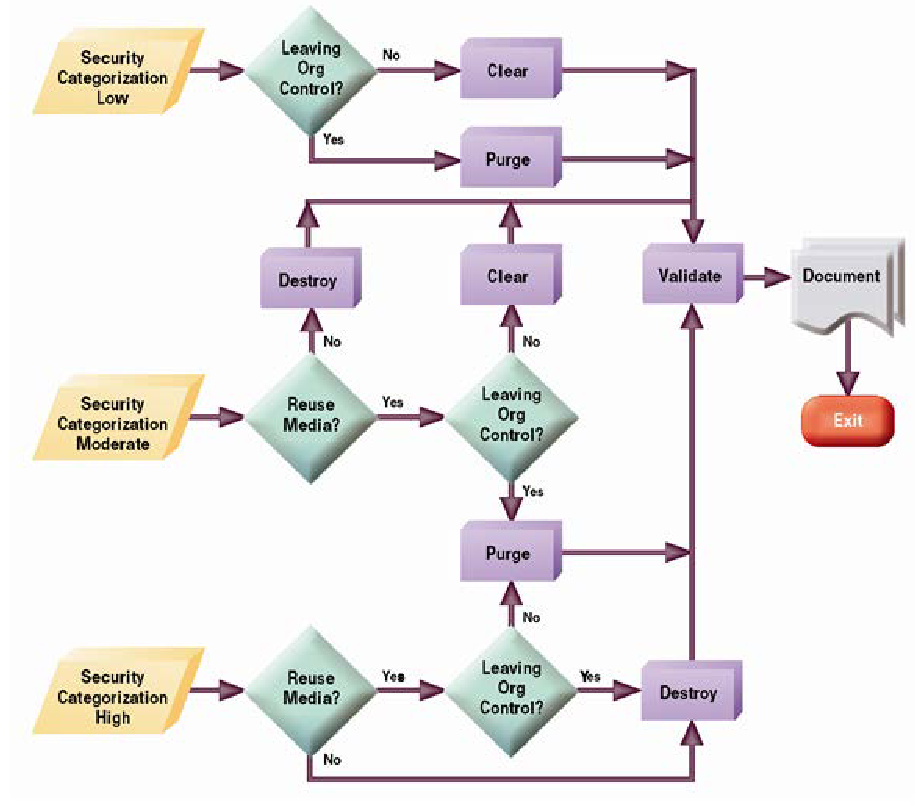
\includegraphics[width=\textwidth]{screen1.png}
\end{column}
\begin{column}{.7\textwidth}
\begin{enumerate}
 \item $\alpha$-Miner
 \begin{itemize}
    \item 2 MapReduce phases
 \end{itemize}
 \item Flexible Heuristic Miner
 \begin{itemize}
    \item 5 MapReduce phases
 \end{itemize}
\end{enumerate}
\begin{itemize}
  \item Random process, 47 activity types
  \item 5 million traces, 80GB event logs
  \item Three cluster sizes:
  \begin{enumerate}
     \item Single node cluster, 2 CPUs
     \item 10-Node cluster, 2 CPUs each
     \item 10-Node cluster, 10 CPUs each
  \end{enumerate}
\end{itemize}
\end{column}
\end{columns}

\vspace{\baselineskip}
\hrule

\small 
\vspace{\baselineskip}
Source: Evermann, J. (2016) Scalable Process Discovery using Map-Reduce. \emph{IEEE TSC}, 9 (3), 469-481. \footnotesize \url{https://doi.org/10.1109/TSC.2014.2367525}
\end{frame}

\begin{frame}{Example -- Flexible Heuristic Miner MapReduce Pipeline}

\begin{itemize}
\item Keys and values can be complex
\item Define a comparison function to shuffle
\end{itemize}
\footnotesize
\begin{align*}
\text{map1:} &(Int, Text) \rightarrow set(CaseID, (Event, TimeStamp)) \\
\text{shuffle1:} &set(caseID, (Event, TimeStamp)) \rightarrow (CaseID, set(Event, TimeStamp)) \\
\text{reduce1:}  &(CaseID, set(Event, TimeStamp)) \rightarrow set((Event, Event), (Int, Bool, Int)) \\
\text{combine2:} &set((Event, Event), (Int, Bool, Int)) \rightarrow set((Event, Event, (Int, Bool, Int)) \\
\text{reduce2:}   &((Event, Event), set(Int, Bool, Int)) \rightarrow set(c, (Event, Event, Int, Float)) \\
\text{reduce3:}  & set(c, (Event, Event), set(Int, Float)) \rightarrow set(c, (Event, Event)) \\
\text{map4:}     & (Int, Text) \rightarrow set(CaseID, (Event, TimeStamp)) \\
\text{shuffle4:} & set(CaseID, (Event, TimeStamp)) \rightarrow (CaseID, set(Event, TimeStamp)) \\
\text{reduce4:}  & (CaseID, set(Event, TimeStamp)) \rightarrow set((Event, set(Event), Bool), Int) \\
\text{reduce5:}  & ((Event, set(Event), Bool), set(Int)) \rightarrow ((Event, set(Event), Bool), Int) 
\end{align*}
\end{frame}

\begin{frame}{MapReduce Use Case -- Results}
\begin{center}
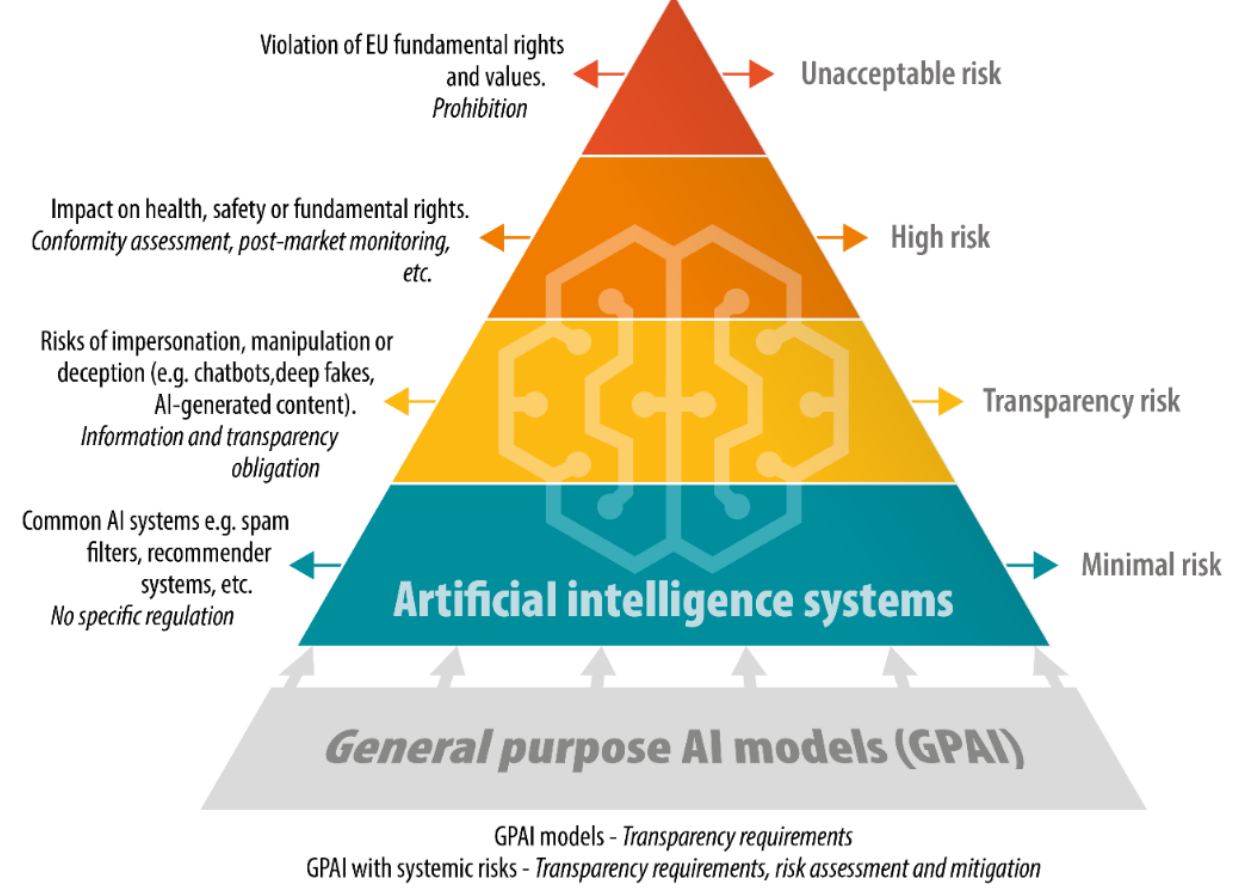
\includegraphics[width=.9\textwidth]{screen2.png} \\
\scriptsize
\vspace{\baselineskip}
Source: Evermann, J. (2016) Scalable Process Discovery using Map-Reduce. \emph{IEEE TSC}, 9 (3), 469-481. \footnotesize \url{https://doi.org/10.1109/TSC.2014.2367525}
\end{center}
\small
\begin{columns}
\begin{column}{.47\textwidth}
\begin{block}{$\alpha$ Algorithm}
\begin{tabular}{lr} \hline
Single node & 25:00 hours \\
Medium cluster & 1:24 hours \\
Large cluster & 0:08 hours \\ \hline
\end{tabular}
\end{block}
\end{column}

\begin{column}{.47\textwidth}
\begin{block}{FHM}
\begin{tabular}{lr} \hline
Single node & 22:21 hours\\
Medium cluster & 2:01 hours \\
Large cluster & 0:17 hours \\ \hline
\end{tabular}
\end{block}
\end{column}
\end{columns}
\end{frame}


\begin{frame}{Apache Pig}
\begin{columns}
\begin{column}{.3\textwidth}
\centering
\includegraphics[width=\textwidth]{pig_logo.png} \\
\tiny\url{https://en.wikipedia.org/wiki/File:Apache_Pig_Logo.svg}
\end{column}
\begin{column}{.7\textwidth}
\begin{itemize}
   \item High-level programming
   \item Pig Latin language
   \item Pig Latin programs run as MapReduce jobs on Hadoop
   \item Procedural, not declarative (SQL)
\end{itemize}

\vspace{\baselineskip}
\url{https://pig.apache.org/docs/latest/basic.html}
\end{column}
\end{columns}
\end{frame}

\begin{frame}[fragile]{Apache Pig Latin Example -- Word Count}
\begin{sqlcode}
input_lines = LOAD 'hamlet.txt' AS (line:chararray);
-- Extract words from each line and put them into 
-- a pig bag datatype, then flatten the bag to get
-- one word on each row
words = FOREACH input_lines \
   GENERATE FLATTEN(TOKENIZE(line)) AS word;
-- create a group for each word
word_groups = GROUP words BY word;
-- count the entries in each group
word_count = FOREACH word_groups  \
   GENERATE COUNT(words) AS count, group AS word;
-- order the records by count
ordered_word_count = ORDER word_count BY count DESC;
STORE ordered_word_count INTO 'hamlet.out';
\end{sqlcode}
\small Source: \url{https://en.wikipedia.org/wiki/Apache_Pig}
\end{frame}

\begin{frame}{Apache Pig Latin -- Relational Operators}
\renewcommand{\arraystretch}{1.5}

\begin{tabular}{ccc} 
LOAD & STORE & DUMP \\
FILTER & DISTINCT & FOREACH $\ldots$ GENERATE \\
SAMPLE & JOIN & GROUP  \\
CROSS & ORDER & LIMIT  \\
UNION & SPLIT \\
\end{tabular}
\end{frame}

\begin{frame}{Apache Hive}
\begin{columns}
\begin{column}{.4\textwidth}
\centering
\includegraphics[width=.75\textwidth]{hive_logo.png} \\
\tiny\url{https://commons.wikimedia.org/wiki/File:Apache_Hive_logo.svg}
\end{column}
\begin{column}{.6\textwidth}
\begin{itemize}
   \item Data warehouse
   \item HiveQL similar to SQL
   \item Translate HiveQL to run as MapReduce jobs on Hadoop
\end{itemize}

\vspace{\baselineskip}
\url{https://cwiki.apache.org/confluence/display/Hive/LanguageManual}
\end{column}
\end{columns}
\end{frame}

\begin{frame}[fragile]{HiveQL Example -- Word Count}
\begin{sqlcode}
DROP TABLE IF EXISTS docs;
CREATE TABLE docs (line STRING);
LOAD DATA INPATH 'hamlet.txt' 
  OVERWRITE INTO TABLE docs;
  
CREATE TABLE word_counts AS
SELECT word, count(1) AS count FROM
  (SELECT explode(split(line, '\s')) 
    AS word FROM docs) temp
GROUP BY word
ORDER BY word;
\end{sqlcode}
\small Source: \url{https://en.wikipedia.org/wiki/Apache_Hive}
\end{frame}

\begin{frame}{Apache Spark}
\begin{columns}
\begin{column}{.4\textwidth}
\includegraphics[width=\textwidth]{spark_logo.png}
\tiny \url{https://commons.wikimedia.org/wiki/File:Apache_Spark_logo.svg} \normalsize
\end{column}
\begin{column}{.6\textwidth}
\begin{itemize}
    \item Origin at UC Berkeley in 2009
    \item Donated to Apache Software Foundation in 2013
    \item Quickly adopted due to performance advantages over MapReduce
    \item Builds on Hadoop HDFS and YARN
    \item Can use other file storage (S3, Azure, etc.) and cluster managers (Mesos, Kubernetes, etc.)
\end{itemize}
\end{column}
\end{columns}
\end{frame}

\begin{frame}{Apache Spark -- Characteristics}
\small
\begin{itemize}
    \item \textbf{In-Memory Processing} with spill-over to disk
    \item \textbf{Efficiency} and much faster processing speed compared to MapReduce.
    \item \textbf{Integration} with Hadoop and its components
    \item \textbf{Unified Engine} for batch processing, real-time streaming, machine learning, and graph processing
    \item \textbf{Advanced Analytics} for machine learning, graph processing, SQL and structured data processing
    \item \textbf{Language Support} for Java, Scala, Python, and R
    \item \textbf{Scalability} from a single server to thousands of nodes.
    \item \textbf{Fault Tolerance} through execution engine that provides ''lineage'' information to recompute lost data
    \item \textbf{Ease of Use} allows quicker development than Hadoop's MapReduce.
\end{itemize}
\end{frame}

\begin{frame}{Apache spark -- Main Components}
\centering
\includegraphics[width=.8\textwidth]{spark_components.png}
\scriptsize \url{https://commons.wikimedia.org/wiki/File:Sch\%C3\%A9ma_d\%C3\%A9tail_outils_spark.png} \normalsize
\end{frame}

\begin{frame}{Apache Spark -- Cluster Overview}
\begin{center}
\includegraphics[width=.8\textwidth]{cluster-overview.png}
\scriptsize \url{https://spark.apache.org/docs/latest/img/cluster-overview.png}
\end{center}
\end{frame}

\begin{frame}{Apache Spark -- Spark on Hadoop}
\begin{itemize}
   \item YARN manages resources for Spark applications
   \item Spark RDD partitions correspond to HDFS blocks
   \item Spark is location aware, schedules job execution on nodes close to data
   \item Two layers of fault tolerance: HDFS replication and Spark RDD lineage
\end{itemize}
\end{frame}

\begin{frame}{Apache Spark -- Data Abstractions}
\small
\begin{enumerate}
  \item RDD (''Resilient Distributed Dataset'')
  \begin{itemize}
    \item Dependencies: Data ''lineage'' information; how the RDD is computed; may be used to reconstruct an RDD
    \item Partitions: Split data among executors; parallelize computation, with location info
    \item Low-level programming interface focused on MapReduce
    \item Procedural, no query optimization
  \end{itemize}
  \item DataFrame
  \begin{itemize}
     \item Inspired by Pandas and R data frames
     \item Builds on RDD
     \item Named columns with data types
     \item High-level programming interface
     \item Immutable
     \item Declarative, query optimization (''Catalyst'' query optimizer)
  \end{itemize}
  \item Dataset
  \begin{itemize}
     \item Strongly typed variant of DataFrame for Java and Scala
  \end{itemize}
\end{enumerate}
\end{frame}

\begin{frame}{Apache Spark -- Execution Principles}
\begin{block}{Transformations}
\begin{itemize}
\item Transform a DataFrame into another DataFrame without altering the original (immutability)
\item Examples: \texttt{map()}, \texttt{select()}, \texttt{filter()}, \texttt{groupBy()}, \texttt{orderBy()}, \texttt{join()}
\item Recorded in data lineage
\item \textbf{Lazy evaluation}: Delay execution until \textbf{action} is invoked; allows query optimization
\end{itemize}
\end{block}
\begin{block}{Actions}
\begin{itemize}
\item Returns a result or writes result to storage
\item Does not produce another DataFrame
\item Examples: \texttt{collect()}, \texttt{count()}, \texttt{show()}, \texttt{take()}
\item Triggers execution of transformations
\end{itemize}
\end{block}
\end{frame}

\begin{frame}[fragile]{Apache Spark -- Basics}
Start the local Hadoop cluster (if not already running) and the PySpark console:
\begin{bashcode}
sudo systemctl start hadoop.service
pyspark --master yarn
\end{bashcode}
Read a file from HDFS and get some statistics:
\begin{pythoncode}
textFile = spark.read.text( \
    'hdfs://localhost:9000/user/busi4720/hamlet.txt')
# Number of lines
textFile.count() 
# First row
textFile.first()
# How many lines contain the word Hamlet?
textFile \
    .filter(textFile.value.contains("Hamlet")) \
    .count() 
\end{pythoncode}
\end{frame}
 
%\begin{frame}[fragile]{Apache Spark -- Basics \small [cont'd]}
%Find the longest line by number of words:
%\begin{pythoncode}
%# Import useful functions from Spark SQL:
%from pyspark.sql import functions as sf

%# Split each line and count words as 'numWord', 
%# then aggregate the 'numWords' columns using 'max':
%textFile \
    %.select(sf.size(sf.split(textFile.value, "\s+")) \
        %.name("numWords")) \
    %.agg(sf.max(sf.col("numWords"))) \
    %.collect()
%\end{pythoncode}
%\end{frame}


\begin{frame}[fragile]{Apache Spark -- Basics \small [cont'd]}
Word count example in Pyspark:
\begin{pythoncode}
# Import useful functions from Spark SQL:
from pyspark.sql import functions as sf

wordCounts = textFile \
    .select(sf.explode(sf.split(textFile.value, "\s+")) \
        .alias("word")) \
    .groupBy("word") \
    .count() \
    .orderBy("count")
wordCounts.collect()
\end{pythoncode}
\end{frame}

\begin{frame}{Apache Spark -- Basic Transformations and Actions}
\begin{block}{Transformations (PySpark)}
\centering
\renewcommand{\arraystretch}{1.5}
\begin{tabular}{ccc} 
select() & filter() & where() \\
withColumn() & groupBy() & sort() \\
distinct() & drop() & cov() \\
orderBy() & withColumnRenamed() & union() \\
join()  \\
\end{tabular}
\end{block}

\begin{block}{Actions (PySpark)}
\centering
\renewcommand{\arraystretch}{1.5}
\begin{tabular}{ccc} 
show() & collect() & take() \\
count() & head() & tail() \\
write.csv() & toPandas() & \\
\end{tabular}
\end{block}
\end{frame}

\begin{frame}[fragile]{Apache Spark -- Schemas and DataFrames}
Schema describes the columns of data frames and their types.
\begin{itemize}
   \item No need for Spark to infer types
   \item No need for Spark to read data to infer schema
   \item Error detection when reading data
\end{itemize}
Define a schema using Spark schema DDL:
\begin{pythoncode}
logSchema = \
    'caseID STRING, \
     activity STRING, \
     ts TIMESTAMP'
\end{pythoncode}
\vspace{-\baselineskip}
\begin{block}{\small Spark DDL Data Types}
\begin{center}
\renewcommand{\arraystretch}{1.5}
\footnotesize
\begin{tabular}{cccc} 
STRING & TINYINT & SMALLINT & INT \\
BIGINT & BOOLEAN & FLOAT & DOUBLE \\
DATE & DECIMAL & TIMESTAMP & BINARY \\ \hline
STRUCT & ARRAY & MAP \\
\end{tabular}
\end{center}
\end{block}
\end{frame}


\begin{frame}[fragile]{Apache Spark -- Schemas and DataFrames}
Read the data from HDFS into a data frame:
\begin{pythoncode}
fname='hdfs://localhost:9000/user/busi4720/\
eventlog.short.log'

data = spark.read \
    .format('csv') \
    .option('delimiter', '\t') \
    .option('header', 'false') \
    .schema(logSchema) \
    .load(fname)
\end{pythoncode}
Query the schema, count rows, show 5 rows, and a summary:
\begin{pythoncode}
data.printSchema()
data.count()
data.show(5)
data.summary().show()
\end{pythoncode}
\end{frame}


\begin{frame}[fragile]{Apache Spark -- SQL}
\small
Register a data frame as a temporary SQL table (''view''):
\begin{pythoncode}
data.createOrReplaceTempView('log')
\end{pythoncode}
Alternatively, create a permanent SQL table:
\begin{pythoncode}
data.write.saveAsTable('log_table')
\end{pythoncode}
Query the SQL table, will return a data frame:
\begin{pythoncode}
result_df = spark.sql('select * from log limit 5')
result_df.show()
\end{pythoncode}
\end{frame}

\begin{frame}[fragile]{Apache Spark -- SQL}
Create a Directly-Follows-Graph (DFG) from a log. Define the SQL Query:
\begin{pythoncode}
sql_query = \
'SELECT COUNT(*), l1.activity AS activity1, \
 l2.activity AS activity2, AVG(l2.ts - l1.ts) AS dtime \
  FROM log AS l1 JOIN log AS l2 ON l1.caseid=l2.caseid \
   WHERE l2.ts = (SELECT MIN(ts) FROM log l3 \
    WHERE l3.caseid=l1.caseid AND l3.ts > l1.ts) \
     GROUP BY GROUPING SETS((l1.activity, l2.activity))'
\end{pythoncode}
Run the query, show the results and explain the query plan:
\begin{pythoncode}
dfg = spark.sql(sql_query)
dfg.count()
dfg.show()

dfg.explain(mode='formatted')
dfg.explain(True)
\end{pythoncode}
\end{frame}

\begin{frame}[fragile]{Apache Spark -- SQL}
Run as self-contained application:
\begin{bashcode}
# Download file
wget https://evermann.ca/busi4720/spark_dfg.py
# Submit to Spark/Hadoop cluster
spark-submit --master yarn spark_dfg.py \
 hdfs://localhost:9000/user/busi4720/eventlog.short.log
\end{bashcode}
Result will be written to HDFS. \\

\begin{block}{Job Tracker}
\begin{center}
Use Hadoop Job Tracker at \url{https://localhost:8088} to track status of nodes and progress of jobs.
\end{center}
\end{block}
\end{frame}

\begin{frame}[fragile]{Apache Spark -- Compare to PostgreSQL}
\begin{bashcode}
psql
\end{bashcode}
Create table and read data from CSV file:
\begin{sqlcode}
CREATE TABLE log(
  caseId VARCHAR(20), 
  activity VARCHAR(10), 
  ts TIMESTAMP);
\COPY log FROM 'eventlog.short.log' 
  WITH DELIMITER E'\t';
\end{sqlcode}
Execute query:
\begin{sqlcode}
SELECT COUNT(*), l1.activity, l2.activity, 
 AVG(l2.ts - l1.ts) AS dtime 
  FROM log AS l1 JOIN log AS l2 ON l1.caseid=l2.caseid 
   WHERE l2.ts = (SELECT MIN(ts) FROM log l3 
    WHERE l3.caseid=l1.caseid AND l3.ts > l1.ts) 
     GROUP BY (l1.activity, l2.activity);
\end{sqlcode}
\end{frame}

\begin{frame}{Apache Spark -- ML}
\begin{block}{Spark ML Frameworks}
\begin{itemize}
   \item \textbf{Spark.mllib}: RDD focused, maintenance only
   \item \textbf{Spark.ml}: Dataframe focused, actively developed
\end{itemize}
\end{block}
\begin{block}{Spark ML Techniques}
\begin{itemize}
   \item \textbf{Supervised}: Classification, Regression
   \item \textbf{Unsupervised}: Clustering, Principal Component Analysis, etc.
\end{itemize}
\end{block}
\end{frame}

\begin{frame}{Apache Spark -- ML Pipelines}
\begin{itemize}
   \item \textbf{Transformers}: Accept a dataframe, execute \texttt{transform()} method, return a dataframe
   \item \textbf{Estimators}: Accept a dataframe, execute \texttt{fit()} method, return a transformer
\end{itemize}
\vspace{.5\baselineskip}
\hrule
\vspace{.5\baselineskip}
\centering
\includegraphics[width=.75\textwidth]{ml-Pipeline1.png} 

\vspace{.5\baselineskip}

\hrule

\vspace{.5\baselineskip}

\includegraphics[width=.75\textwidth]{ml-Pipeline2.png} 

\scriptsize \url{https://spark.apache.org/docs/latest/ml-pipeline.html} \normalsize
\end{frame}


\begin{frame}{Apache Spark -- Selection of available ML Models}
\begin{block}{\small Classification}
\begin{center}
\renewcommand{\arraystretch}{1.5}
\footnotesize
\begin{tabular}{ccc} 
Logistic regression & Decision trees & Random forests \\
Gradient-boosted trees & Multilayer perceptron & Support vector machines \\
& Naive bayes
\end{tabular}
\end{center}
\end{block}
\begin{block}{\small Regression}
\begin{center}
\renewcommand{\arraystretch}{1.5}
\footnotesize
\begin{tabular}{cc} 
Linear regression & Generalized linear regression \\
Decision tree regression & Random forest regression \\
GBT regression & Survival regression \\
\end{tabular}
\end{center}
\end{block}
\begin{block}{\small Unsupervised}
\begin{center}
\renewcommand{\arraystretch}{1.5}
\footnotesize
\begin{tabular}{cccc} 
K-means clustering & Principal components \\
\end{tabular}
\end{center}
\end{block}
\end{frame}

%\begin{frame}[fragile]{Apache Spark -- ML Pipelines}
%Get the dataset:
%\begin{bashcode}
%wget https://evermann.ca/busi4720/mushrooms.csv
%hdfs dfs -put mushrooms.csv
%\end{bashcode}
%\scriptsize Source: 
%\url{https://archive.ics.uci.edu/dataset/848/secondary+mushroom+dataset} \\ CC-BY 4.0 license \\

%\normalsize Define the schema:
%\begin{pythoncode}
%wine_schema = 'fixed_acidity FLOAT, \
    %volatile_acidity FLOAT, citric_acid FLOAT, \
    %residual_sugar FLOAT, chlorides FLOAT, \
    %free_sulfur_dioxide FLOAT, \
    %total_sulfur_dioxide FLOAT, \
    %density FLOAT, PhD FLOAT, \
    %sulphates FLOAT, alcohol FLOAT, \
    %quality INT'
%\end{pythoncode}
%\end{frame}

%\begin{frame}[fragile]{Apache Spark -- ML Pipelines}
%Load data:
%\begin{pythoncode}
%fname='hdfs://localhost:9000/user/busi4720/\
%winequality-white.csv'

%data = spark.read \
    %.format('csv') \
    %.option('header', 'true') \
    %.schema(wine_schema) \
    %.load(fname)
%\end{pythoncode}
%\end{frame}


\begin{frame}[fragile]{Apache Spark -- ML Example}
Full example at \small\url{https://evermann.ca/busi4720/spark_ml.py}\normalsize \\

Run as self-contained application:
\begin{bashcode}
# Download file
wget https://evermann.ca/busi4720/spark_ml.py
# Submit to Spark/Hadoop cluster
spark-submit --master yarn spark_ml.py \
    hdfs://localhost:9000/user/busi4720/mushrooms.csv
\end{bashcode}

\begin{block}{Job Tracker}
\begin{center}
Use Hadoop Job Tracker at \url{https://localhost:8088} to track status of nodes and progress of jobs.
\end{center}
\end{block}
\end{frame}

\begin{frame}[fragile]{Apache Spark -- ML Example}
Get the dataset:
\begin{bashcode}
wget https://evermann.ca/busi4720/mushrooms.csv
hdfs dfs -put mushrooms.csv
\end{bashcode}
\tiny \url{https://archive.ics.uci.edu/dataset/848/secondary+mushroom+dataset} \\ CC-BY 4.0 license \\

\normalsize Define the schema:
\begin{pythoncode}
the_schema = 'class STRING, `cap-diameter` DOUBLE, \
    `cap-shape` STRING, `cap-surface` STRING, \
    `cap-color` STRING, `does-bruise-or-bleed` STRING, \
    `gill-attachment` STRING, `gill-spacing` STRING, \
    `gill-color` STRING, `stem-height` DOUBLE, \
    `stem-width` DOUBLE, `stem-root` STRING, \
    `stem-surface` STRING, `stem-color` STRING, \
    `veil-type` STRING, `veil-color` STRING, \
    `has-ring` STRING, `ring-type` STRING, \
    `spore-print-color` STRING, habitat STRING, \
    season STRING'
\end{pythoncode}
\end{frame}

\begin{frame}[fragile]{Apache Spark -- ML Example}
Load data:
\begin{pythoncode}
fname='hdfs://localhost:9000/user/busi4720/\
mushrooms.csv'

data = spark.read \
    .format('csv') \
    .option('delimiter', ',') \
    .option('header', 'true') \
    .schema(the_schema) \
    .load(fname)
data = data.drop('veil-type')
data = data.fillna('NULL')
\end{pythoncode}
\end{frame}

\begin{frame}[fragile]{Apache Spark -- ML Example}
Import all required pieces:
\begin{pythoncode}
from pyspark.ml import Pipeline
from pyspark.ml.classification import LogisticRegression
from pyspark.ml.feature import StandardScaler, \
    StringIndexer, OneHotEncoder, VectorAssembler
from pyspark.ml.evaluation \
    import BinaryClassificationEvaluator
from pyspark.ml import PipelineModel
\end{pythoncode}
Create the necessary \textbf{transformers} for the pipeline. Collect all numerical features:
\begin{pythoncode}
numFeatures = VectorAssembler(
    inputCols = ['cap-diameter', 'stem-width', 
                 'stem-height'],
    outputCol = 'numFeatures')

scaler = StandardScaler(inputCol='numFeatures',
                        outputCol='numFeaturesS')
\end{pythoncode}
\end{frame}

\begin{frame}[fragile]{Apache Spark -- ML Example}
Encode categorical variables as one-hot (dummy variables):
\begin{pythoncode}
categoricalCols = \
    [name for (name, dtype) in data.dtypes \
        if dtype=='string']
indexOutputCols = \
    [x + 'index' for x in categoricalCols]
oheOutputCols = \
    [x + 'ohe' for x in categoricalCols]

stringIndexer = StringIndexer(
    inputCols = categoricalCols,
    outputCols = indexOutputCols,
    handleInvalid='skip')

oheEncoder = OneHotEncoder(
    inputCols = indexOutputCols,
    outputCols = oheOutputCols)
\end{pythoncode}
\end{frame}

\begin{frame}[fragile]{Apache Spark -- ML Example}
Assemble all features into a feature vector:
\begin{pythoncode}
vecAssembler = VectorAssembler(
    inputCols = oheOutputCols+['numFeaturesS'],
    outputCol = 'feature_vec')
\end{pythoncode}
Encode the target classes as numbers:
\begin{pythoncode}
stringIndexTarget = StringIndexer(
    inputCols = ['class'],
    outputCols = ['classIndex'],
    handleInvalid='skip')
\end{pythoncode}    
Create the classification \textbf{estimator}:
\begin{pythoncode}
logReg = LogisticRegression(
    featuresCol = 'feature_vec',
    labelCol = 'classIndex')
\end{pythoncode}
\end{frame}

\begin{frame}[fragile]{Apache Spark -- ML Example}
Put all components into the \textbf{pipeline}:
\begin{pythoncode}
pipeline = Pipeline(stages=[
    numFeatures,
    scaler,
    stringIndexer,
    oheEncoder,
    vecAssembler,
    stringIndexTarget,
    logReg])
\end{pythoncode}
\end{frame}


\begin{frame}[fragile]{Apache Spark -- ML Example}
Create train/test data split:
\begin{pythoncode}
train_data, test_data = \
    data.randomSplit([.66, .33], seed=1)
\end{pythoncode}
Fit the model to the training data:
\begin{pythoncode}
pipelineModel = pipeline.fit(train_data)
\end{pythoncode}
Summary of the training data:
\begin{pythoncode}
summary = pipelineModel.stages[-1].summary
summary.accuracy
summary.areaUnderROC
summary.fMeasureByThreshold.show()
summary.precisionByLabel
summary.recallByLabel
summary.roc.show()
\end{pythoncode}
\end{frame}

\begin{frame}[fragile]{Apache Spark -- ML Example}
Fitted estimators (including whole pipelines) become transformers. Predict for both training and testing data:
\begin{pythoncode}
trainPred = pipelineModel.transform(train_data)
testPred = pipelineModel.transform(test_data)
\end{pythoncode}
Evaluate the model using AUC:
\begin{pythoncode}
evaluator = BinaryClassificationEvaluator(
    labelCol='classIndex')
evaluator.evaluate(trainPred)
evaluator.evaluate(testPred)
\end{pythoncode}
Save the fitted model for later re-use:
\begin{pythoncode}
pipelineModel.write().overwrite().save('myFirstModel')
\end{pythoncode}
Load a saved model:
\begin{pythoncode}
savedModel = PipelineModel.load('myFirstModel')
\end{pythoncode}
\end{frame}


\begin{frame}{Stream Analytics}
\begin{itemize}
    \item Network (''directed acyclic graph'') of nodes
    \item Ingest records, process records, emit records
    \item Record-by-record processing
    \item Low latencies
    \item Resource intensive
\end{itemize}
\begin{block}{Example Use Cases}
\begin{itemize}
   \item Customer click-stream analysis for real-time pricing
   \item Machine sensor data for failure warnings/alarms
   \item Financial/payments transaction fraud monitoring
   \item Market data anlytics, news monitoring
   \item Activity records for process compliance monitoring
   \item \ldots
\end{itemize}
\end{block}

\end{frame}

\begin{frame}{Process Discovery with Streaming Data}
\begin{columns}
\begin{column}{.3\textwidth}
\includegraphics[width=\textwidth]{cloudcom_logo.png}
\end{column}
\begin{column}{.7\textwidth}
\begin{itemize}
   \item Flexible Heuristics Miner
   \item Activity completion records
   \item Record-by-record processing
   \item 57,000 -- 160,000 traces per min
   \item 2,000,000 -- 5,500,000 events per min
   \item 5 16-core, 32GB nodes
\end{itemize}
\end{column}
\end{columns}
\vspace{\baselineskip}

\hrule

\vspace{\baselineskip}

\footnotesize
Source: Evermann, J., Rehse, J.-R., and Fettke, P.: Process Discovery from Event Stream Data in the Cloud - A Scalable, Distributed Implementation of the Flexible Heuristics Miner on the Amazon Kinesis Cloud Infrastructure. \emph{CloudBPM Workshop on Business Process Monitoring and Performance Analysis in the Cloud at the 8th IEEE International Conference on Cloud Computing Technologies and Science (CloudCom 2016)} .
\end{frame}

\begin{frame}{Process Discovery with Streaming Data}
\begin{columns}
\begin{column}{.4\textwidth}
\includegraphics[height=3in]{screen3.png}
\end{column}
\begin{column}{.6\textwidth}
\begin{itemize}
   \item Implemented on AWS Kinesis
   \item Directed acyclic graph (DAG)
   \item Multiple event generators
   \item Multiple record streams
   \item Stream is queue with ''Put'' and ''Read'' operations
   \item Streams contain multiple ''shards'' (same keys)
   \item Multiple threads/executors per shard (key)
\end{itemize}
\end{column}
\end{columns}
\end{frame}

\begin{frame}{Process Discovery with Streaming Data}
Performance Results:
\begin{center}
\includegraphics[width=\textwidth]{screen4.png}
\end{center}
\end{frame}

\begin{frame}{Apache Spark -- Stream Analytics}
\begin{block}{Principles}
\begin{itemize}
    \item Micro-batches
    \item Data stream as unbounded dataframe/table
    \item Unified programming model for batch and stream processing
    \item Support for time windows
    \item Wide range of input sources and output destinations
    \item Optimized stateful stream transformations and aggregations
\end{itemize}
\end{block}
\end{frame}

\begin{frame}{Apache Spark -- Stream Analytics}
\centering

\includegraphics[width=.8\textwidth]{streaming-arch.png} \\
\scriptsize\url{https://spark.apache.org/docs/latest/img/streaming-arch.png}\normalsize \\

\vspace{\baselineskip}

\hrule

\vspace{\baselineskip}

\includegraphics[height=1in]{streaming-flow.png}  \\

\scriptsize\url{https://spark.apache.org/docs/latest/img/streaming-flow.png}
\end{frame}

\begin{frame}{Apache Spark -- Stream Analytics}
\includegraphics[width=\textwidth]{stream-as-a-table.png} \\

\scriptsize\url{https://spark.apache.org/docs/latest/img/structured-streaming-stream-as-a-table.png}
\end{frame}

\begin{frame}{Apache Spark -- Stream Analytics}
\begin{block}{Triggering}
\begin{itemize}
   \item Micro-batch (process next batch when prior batch completed)
   \item Time trigger
   \item Once
   \item Continuous
\end{itemize}
\end{block}
\begin{block}{Output Modes}
\begin{itemize}
   \item Append: Assume older output remains valid
   \item Update: Change parts of older output (requires appropriate output destination, e.g. PostgreSQL, but not HDFS)
   \item Complete: Replace/overwrite older output
\end{itemize}
\end{block}
\end{frame}

%\begin{frame}{Apache Spark -- Stream Analytics}
%\includegraphics[width=\textwidth]{structured-streaming-model.png} \\

%\scriptsize\url{https://spark.apache.org/docs/latest/img/structured-streaming-model.png}
%\end{frame}

\begin{frame}[fragile]{Apache Spark -- Stream Analytics}
Import all necessary functions and get a Spark Session:
\begin{pythoncode}
from pyspark.sql.functions import \
    explode, split, col, desc, \
    window, current_timestamp
\end{pythoncode}
Create the stream reader to read from a network socket:
\begin{pythoncode}
lines = spark.readStream \
             .format('socket') \
             .option('host', 'localhost') \
             .option('port', 9999) \
             .load()
\end{pythoncode}
\texttt{lines} is a DStream. \\

The stream reader opens a \emph{client} socket, i.e. the socket must already be opened for writing.
\end{frame}

\begin{frame}[fragile]{Apache Spark -- Stream Analytics}
Define processing of lines:
\begin{pythoncode}
words = lines.select(explode(split(col('value'), \
    '\\s')).alias('word'))
\end{pythoncode}
\texttt{words} is another DStream, connected to \texttt{lines} \\

\includegraphics[width=\textwidth]{streaming-dstream-ops.png}
\scriptsize\url{https://spark.apache.org/docs/latest/img/streaming-dstream-ops.png}\normalsize

\end{frame}


\begin{frame}[fragile]{Apache Spark -- Stream Analytics}
Define processing of words:
\begin{pythoncode}
counts = words.groupBy('word') \
              .count() \
              .sort(desc('count'))
\end{pythoncode}
\texttt{counts} is another Dstream, connected to \texttt{words} \\

Define the output writer with output mode and processing trigger:
\begin{pythoncode}
writer = counts.writeStream \
           .format('console') \
           .outputMode('complete') \
           .trigger(processingTime='5 second') \
           .option('checkpointLocation', \
               'hdfs://localhost:9000/user/busi4720/')
\end{pythoncode}
\end{frame}

\begin{frame}{Apache Spark -- Stream Analytics}
\includegraphics[width=\textwidth]{structured-streaming-example-model.png} \\

\scriptsize\url{https://spark.apache.org/docs/latest/img/structured-streaming-example-model.png}
\end{frame}

\begin{frame}[fragile]{Apache Spark -- Stream Analytics}
First, open a server socket from the shell using \texttt{nc}:
\begin{bashcode}
nc -kl 9999
\end{bashcode}
Start the processing by starting the writer. This returns a streaming query object that provides progress information. ''\texttt{start()}'' is a non-blocking operation:
\begin{pythoncode}
streamingQuery = writer.start()
\end{pythoncode}
\end{frame}


\begin{frame}[fragile]{Apache Spark -- Stream Analytics}
Get progress information through the \texttt{lastProgress} attribute of the query:
\begin{pythoncode}
print(streamingQuery.lastProgress)
\end{pythoncode}
Stop the processing by calling \texttt{stop()} on the query object:
\begin{pythoncode}
streamingQuery.stop()
\end{pythoncode}
\end{frame}

\begin{frame}[fragile]{Apache Spark -- Stream Analytics}
\begin{block}{Fault Tolerance}
\begin{itemize}
   \item Checkpointing of state
   \item ''End-to-end exactly-once'' guarantees
   \begin{itemize}
       \item Replayable sources
       \item Deterministic computations   
       \item Destination that can identify duplicates
   \end{itemize}
\end{itemize}
\end{block}
\end{frame}

\begin{frame}[fragile]{Apache Spark -- Stream Analytics}
\begin{block}{Time Windowing}
\begin{pythoncode}
words = lines.select(explode(split(col('value'), \
    '\\s')).alias('word')) \
    .withColumn('eventTime', current_timestamp())

counts = words \
    .groupBy('word', \
        window('eventTime', '1 minute', '30 second')) \
    .count() \
    .sort(desc('count'))
\end{pythoncode}
\end{block}
\end{frame}

\begin{frame}{Apache Spark -- Stream Analytics}
\includegraphics[width=\textwidth]{structured-streaming-window.png} \\

\scriptsize\url{https://spark.apache.org/docs/latest/img/structured-streaming-window.png}
\end{frame}


\begin{frame}{Apache Spark -- Stream Analytics}
\begin{enumerate}
   \item Streaming ML Learning
   \begin{itemize}
       \item Streaming Linear Regression
       \item Streaming Logistic Regression
       \item Streaming KMeans
   \end{itemize}
   \item Streaming ML Prediction
   \begin{itemize}
       \item From off-line trained models
   \end{itemize}
\end{enumerate}
\end{frame}

\begin{frame}{Apache Spark -- Further Reading}
\begin{block}{Quick Start}
\footnotesize
\url{https://spark.apache.org/docs/latest/quick-start.html}\normalsize
\end{block}

\begin{block}{SQL, DataFrames and Datasets}
\footnotesize
\url{https://spark.apache.org/docs/latest/sql-programming-guide.html}\normalsize
\end{block}

\begin{block}{Structured Streaming}
\footnotesize
\url{https://spark.apache.org/docs/latest/structured-streaming-programming-guide.html}\normalsize
\end{block}

\begin{block}{Machine Learning}
\footnotesize
\url{https://spark.apache.org/docs/latest/ml-guide.html}\normalsize
\end{block}

\scriptsize Last accessed on March 8, 2024
\end{frame}

\end{document}



